\documentclass{article}

\usepackage[main=english,vietnamese]{babel}
\usepackage[T1]{fontenc}
\usepackage[utf8]{inputenc}
\usepackage[sexy]{evan}
\usepackage{matchsticks}
\usepackage{wrapfig}
\usepackage{listings}

\newtheorem{hint}{Hint}

\title{A picture is worth a thousand words - Part 2}
\author{Nghia Doan}
\date{\today}

\begin{document}

\maketitle

This article is the second part of the series on investigating a number of ways to \textit{prove area equality without writing lengthy proof.}

\begin{example*}[Example 6]
    $ABCD$ is a rectangle. $E, F$ are arbitrary points on of $CD, DA,$ respectively.
    Circle $\omega$ center at $I$ is tangent to sides $BC, CD,$ and diagonal $BD.$
    Lines through $I$ parallel to the sides of the rectangle intersect $AB$ at $E$ and $DA$ at $F.$
    Prove that
    \[
        [AEIF] = \half [ABCD].
    \]
\end{example*}

\begin{figure}[h]
    \centering
    \begin{minipage}[t]{6.5cm}
        \begin{center}
            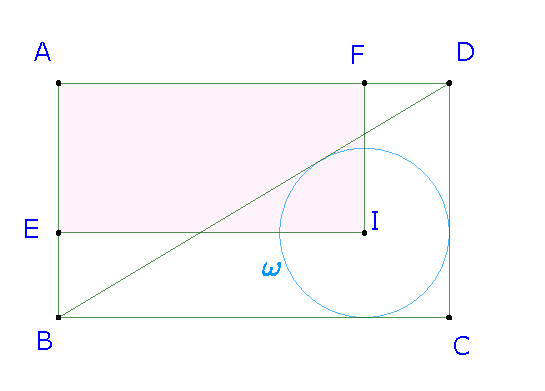
\includegraphics[width=6.5cm]{./svg/pdf/23-24-s3-i-p6.pdf}
        \end{center}
    \end{minipage}
    \qquad
    \begin{minipage}[t]{6.5cm}
        \centering
        \begin{center}
            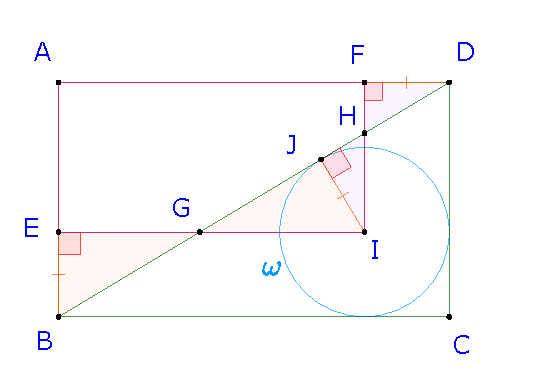
\includegraphics[width=6.5cm]{./svg/pdf/23-24-s3-i-p6-s.pdf}
        \end{center}
    \end{minipage}
\end{figure}

\begin{proof}
    Let $I$ be the tangent point of circle $\omega$ with $BD.$ $\triangle BEG$ and $\triangle CJG$ are both right triangles
    and have the short legs with the same length $EB=IJ$ ($=$ the radius of $\omega$), thus they are congruent and have the same area.
    Similarly $\triangle IJH$ and $\triangle FDH$ have the same area.
    \[ 
        [AEIF] = [AEGHF] + [GIH] = [AEGHF] + [GIJ] + [IJH] = [AEGHF] + [EGB] +  [HFD] = \half [ABCD].
    \]
\end{proof}

\newpage

\begin{example*}[Example 7]
    \label{example:23-24-s3-i-p7}
    $ABCD$ is a parallelogram. $E, F, G,$ and $H$ are midpoints of $AB, BC, CD,$ and $DA,$ respectively.
    Segments $AG, BH, CE, EF$ intersect at $I, J, K,$ and $L,$ as shown below. 
    Prove that the area of the blue region is the same as the sum of the areas of the red regions.
\end{example*}

\begin{figure}[h]
    \centering
    \begin{minipage}[t]{6.5cm}
        \begin{center}
            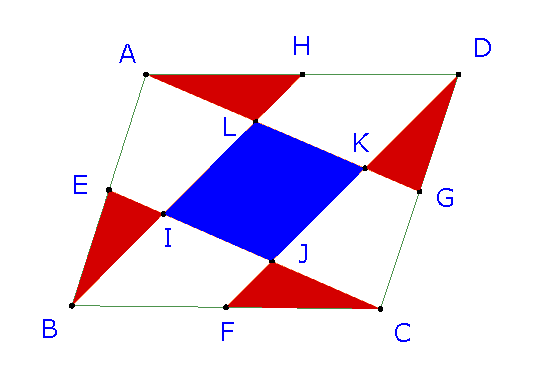
\includegraphics[width=6.5cm]{./svg/pdf/23-24-s3-i-p7.pdf}
        \end{center}
    \end{minipage}
    \qquad
    \begin{minipage}[t]{6.5cm}
        \centering
        \begin{center}
            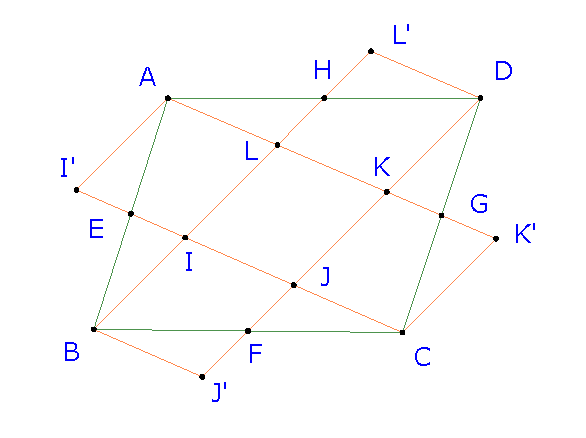
\includegraphics[width=6.5cm]{./svg/pdf/23-24-s3-i-p7-s.pdf}
        \end{center}
    \end{minipage}
\end{figure}

\begin{proof}
    Let $I', J', K', L'$ be the reflections of $I, J, K, L$ over $E, F, G, H,$ respectively.
    It is easy to prove that $ALII',$ $BIJJ',$ $CJKK',$ and $DKLL'$ as well as $IJKL$ are congruent parallelograms.
    Thus, the sum of the area of the red region is equivalent to the area of one of these parallelograms.
\end{proof}

\begin{example*}[Example 8]
    \label{example:23-24-s3-i-p8}
    A half cirle and two quarters of circles are draw in a square as shown below.
    Find the ratio of the area of the shaded region to the area of the square.
\end{example*}

\begin{figure}[h]
    \centering
    \begin{minipage}[t]{6.5cm}
        \begin{center}
            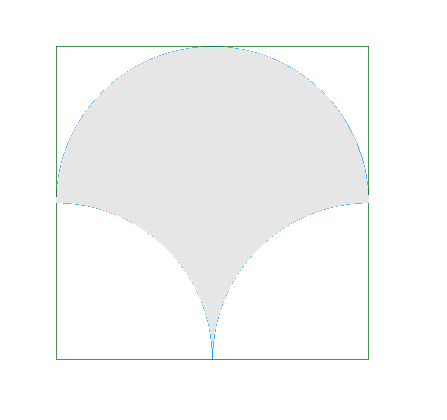
\includegraphics[width=6.5cm]{./svg/pdf/23-24-s3-i-p8.pdf}
        \end{center}
    \end{minipage}
    \qquad
    \begin{minipage}[t]{6.5cm}
        \centering
        \begin{center}
            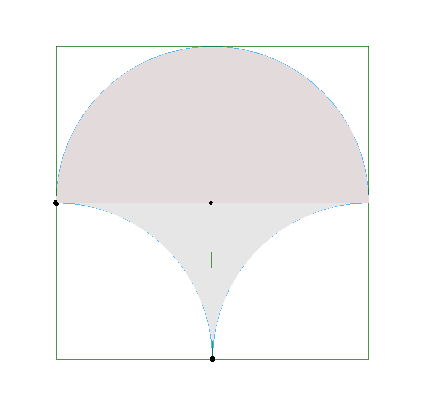
\includegraphics[width=6.5cm]{./svg/pdf/23-24-s3-i-p8-s.pdf}
        \end{center}
    \end{minipage}
\end{figure}

\begin{proof}
    The area of the shaded region contains a half circle plus twice of the difference of a quarter of the square with the area of a quarter circle.
    The half circle and two quarter circles cancel out, leaving twice quarter of the square, thus the ratio is $\frac{1}{2}.$ 
\end{proof}

\newpage

\begin{example*}[Example 9]
    \label{example:23-24-s3-i-p9}
    $\triangle ABC$ is equilateral. Points $E, F$ trisect the side $AB,$ point $GF, H$ trisect the side $BC.$ $IE$ is parallel to $BC.$
    Find the ratio of the shaded area to the area of $\triangle ABC.$
\end{example*}

\begin{figure}[h]
    \centering
    \begin{minipage}[t]{6.5cm}
        \begin{center}
            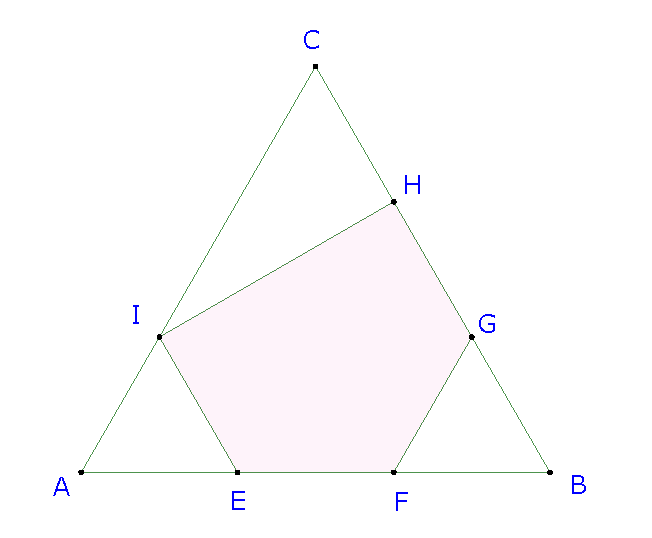
\includegraphics[width=6.5cm]{./svg/pdf/23-24-s3-i-p9.pdf}
        \end{center}
    \end{minipage}
\end{figure}

\begin{proof}
    Since $AE = \frac{1}{3}AB,$ thus $[AIE] = \left(\frac{1}{3}\right)^2[ABC] = \frac{1}{9}[ABC].$  $[BGF] = [AIE].$ 
    $\triangle CHI$ is right triangle at $H,$ $CH = \frac{1}{3} BC,$ $IH$ is two-third of the altitude from $A$ to $BC,$ thus
    $[CIH] = \frac{1}{3}\cdot\frac{2}{3} [ABC].$
    Hence
    \[
        \frac{[EFGHI]}{[ABC]} = 1- \frac{1}{9} - \frac{1}{9} - \frac{2}{9} = \frac{5}{9}.
    \]
\end{proof}

\begin{example*}[Example 10]
    In the hexagon $ABCDEF,$ $AB \parallel DE,$ $BC \parallel EF,$ $CD \parallel FA,$ $AB = DE,$ $BC = EF,$ and $CD = FA.$
    Prove that
    \[
        [BDF] = \half [ABCDEF].
    \]
\end{example*}

\begin{figure}[h]
    \centering
    \begin{minipage}[t]{6.5cm}
        \begin{center}
            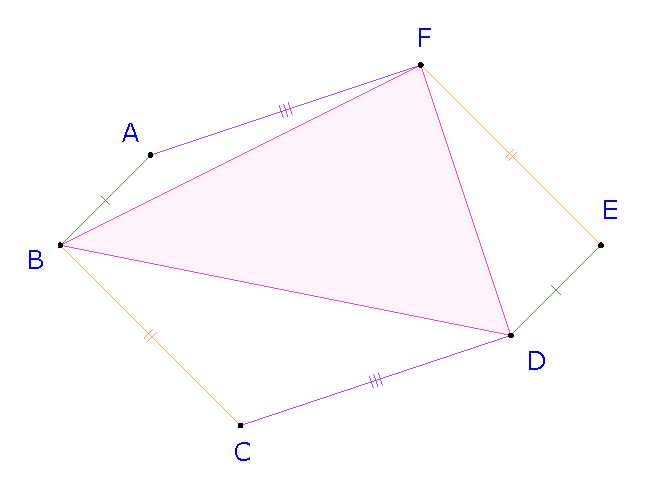
\includegraphics[width=6.5cm]{./svg/pdf/23-24-s3-i-p11.pdf}
        \end{center}
    \end{minipage}
    \qquad
    \begin{minipage}[t]{6.5cm}
        \centering
        \begin{center}
            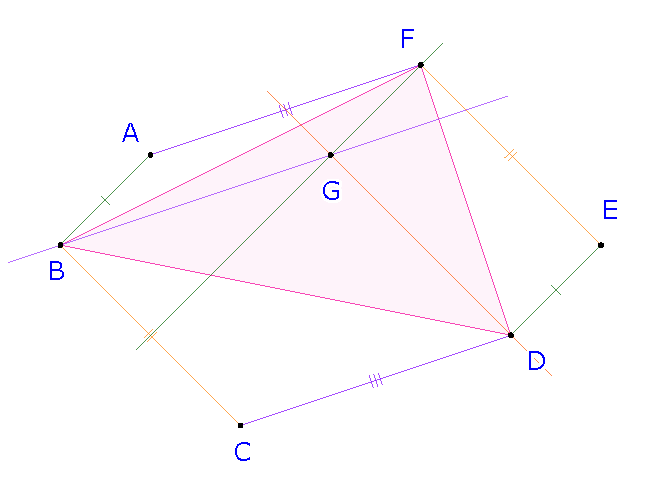
\includegraphics[width=6.5cm]{./svg/pdf/23-24-s3-i-p11-s.pdf}
        \end{center}
    \end{minipage}
\end{figure}

\begin{proof}
    Draw lines through $B$ parallel with $AD$ and $CD,$ through $D$ parallel with $CB$ and $EF,$ through $F$ parallel with $AB$ and $ED.$
    They are concurrent at $G$ (all meet at $G$, can you prove it?) and divide the hexagon into three parallelograms $ABGF,$ $CDGB,$ and $DEFG.$
    They also divide the shaded triangle $BDF$ into three triangles, each's area is half of the parallelogram whose contains it.
    Therefore the area of the shaded triangle is half of the hexagon.
\end{proof}

\end{document}